\section{Methodology}

Let us define the objective function $M$ as 


Nullam mollis in lectus vitae tempus. Nam pellentesque tincidunt leo id dapibus. Etiam in euismod diam. \cite{ceres-solver, Asaro:1976:POT} Phasellus feugiat ante et dui rhoncus, at dictum elit vehicula. Nunc ut finibus neque. Sed vehicula tristique - as shown in Table \ref{soccer} - odio at interdum. Morbi ex lectus, porttitor vel ipsum id, scelerisque facilisis metus. Cras orci sapien, luctus in eros in, suscipit rhoncus neque. Duis pharetra elit vitae sagittis maximus. Curabitur fermentum justo massa, sed placerat odio aliquam quis. Nam facilisis hendrerit ante eget maximus. Nulla et porttitor nibh, et malesuada turpis. Suspendisse potenti. Nunc ultricies suscipit quam, eget ultrices nisi viverra vitae.

\begin{table}[ht]
\begin{center}
    \caption{Soccer, or football?}
\label{soccer}
\begin{tabular}{l*{6}{c}r}
Team              & P & W & D & L & F  & A & Pts \\
\hline
Manchester United & 6 & 4 & 0 & 2 & 10 & 5 & 12  \\
Celtic            & 6 & 3 & 0 & 3 &  8 & 9 &  9  \\
Benfica           & 6 & 2 & 1 & 3 &  7 & 8 &  7  \\
FC Copenhagen     & 6 & 2 & 1 & 3 &  5 & 8 &  7  \\
\end{tabular}
\end{center}
\end{table}

Aliquam sed vehicula neque. Praesent placerat, nisi sit amet condimentum porta, justo tellus dictum eros, quis vestibulum erat massa id sapien. Vestibulum euismod purus dolor, ornare consectetur quam egestas volutpat. Curabitur sollicitudin convallis purus ultrices facilisis. Pellentesque sollicitudin maximus orci quis rutrum. Phasellus a mauris maximus sem mollis sagittis. Vivamus sagittis faucibus tincidunt. Vivamus vel suscipit leo.

\begin{figure}[h]
  \centering
  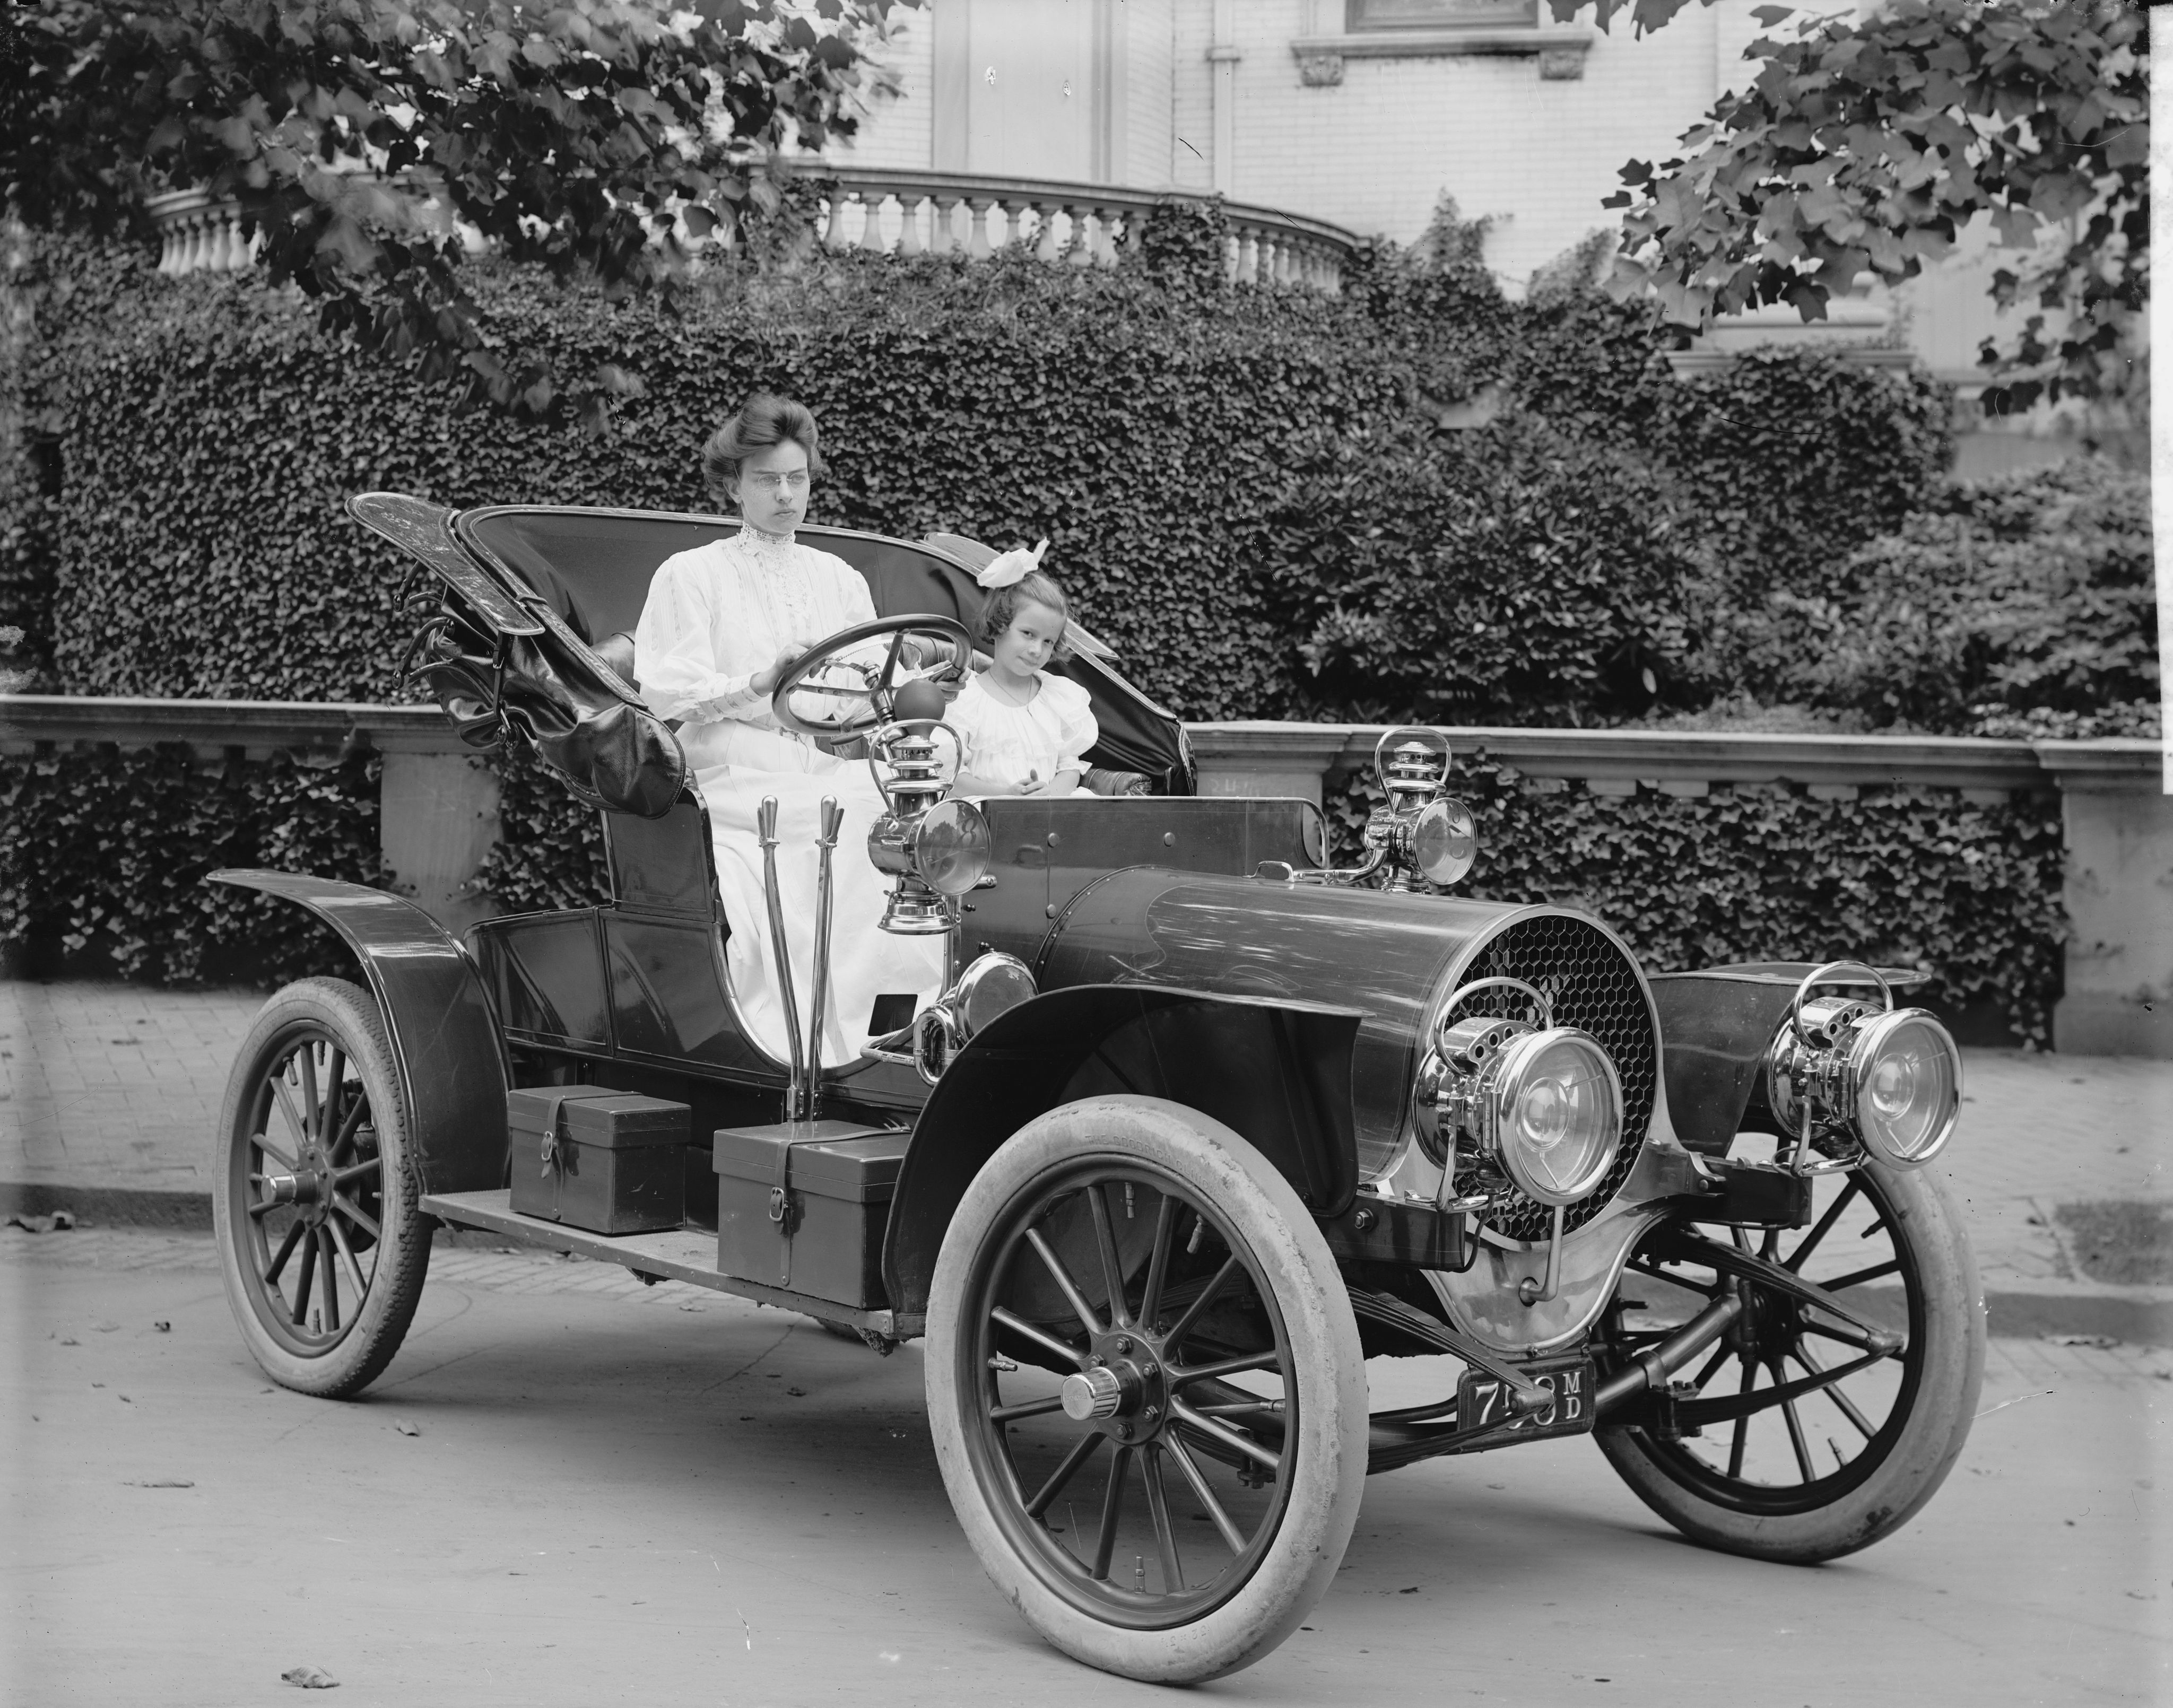
\includegraphics[width=\linewidth]{fig/franklin}
  \caption{1907 Franklin Model D roadster. Photograph by Harris \& Ewing, Inc. [Public domain], via Wikimedia Commons. (\url{https://goo.gl/VLCRBB}).}
\end{figure}